% XeLaTeX can use any Mac OS X font. See the setromanfont command below.
% Input to XeLaTeX is full Unicode, so Unicode characters can be typed directly into the source.

% The next lines tell TeXShop to typeset with xelatex, and to open and save the source with Unicode encoding.

%!TEX TS-program = xelatex
%!TEX encoding = UTF-8 Unicode

\documentclass[10pt]{article}
\usepackage{geometry}                % See geometry.pdf to learn the layout options. There are lots.
\geometry{letterpaper}                   % ... or a4paper or a5paper or ... 
%\geometry{landscape}                % Activate for for rotated page geometry
%\usepackage[parfill]{parskip}    % Activate to begin paragraphs with an empty line rather than an indent
\usepackage{graphicx}
\usepackage{amssymb}
%%%% Package
\usepackage{amsmath,amssymb,amsthm}
\usepackage[UTF8,noindent]{ctex}
\usepackage{pgf}
\usepackage{tikz}
\usetikzlibrary{calc}
\usetikzlibrary{arrows,snakes,backgrounds,shapes,shadows}
\usetikzlibrary{matrix,fit,positioning,decorations.pathmorphing}
\usepackage{listings}
\lstset{
  keywordstyle=\color{blue!70},
  frame=single,
  basicstyle=\ttfamily,
  commentstyle=\small\color{red},
  breakindent=0pt,
  rulesepcolor=\color{red!20!green!20!blue!20},
  rulecolor=\color{black},
  tabsize=4,
  numbersep=5pt,
  breaklines=true,
  %% backgroundcolor=\color{red!10},
  showspaces=false,
  showtabs=false,
  extendedchars=false,
  escapeinside=``,
  frame=no,
}

%%%% New Commands
\newcommand{\blue}{\textcolor{blue}}
\newcommand{\red}{\textcolor{red}}
\newcommand{\purple}{\textcolor{electricpurple}}
\newcommand{\ds}{\displaystyle}
\newcommand{\cd}{\cdots}
\newcommand{\dd}{\ddots}
\newcommand{\vd}{\vdots}
\newcommand{\id}{\iddots}


% Will Robertson's fontspec.sty can be used to simplify font choices.
% To experiment, open /Applications/Font Book to examine the fonts provided on Mac OS X,
% and change "Hoefler Text" to any of these choices.

\usepackage{fontspec,xltxtra,xunicode}
\defaultfontfeatures{Mapping=tex-text}
\setromanfont[Mapping=tex-text]{Hoefler Text}
\setsansfont[Scale=MatchLowercase,Mapping=tex-text]{Gill Sans}
\setmonofont[Scale=MatchLowercase]{Andale Mono}

\begin{document}
\renewcommand{\proofname}{\textbf{证明}}
%%%% New Theorem
\newtheorem{li}{例}
\newtheorem{jielun}{结论}
\newtheorem{dingli}{定理}
\newtheorem{mingti}{{命题}} 
\newtheorem{yinli}{{引理}} 
\newtheorem{tuilun}{{推论}}
\newtheorem{dingyi}{{定义}} 
\newtheorem*{jie}{{解}}
\newtheorem*{zhengming}{{证明}}
\newtheorem{zhu}{{注}}
\newtheorem*{zhu*}{{注}}
\newtheorem{xingzhi}{{性质}}
\newtheorem{wenti}{{问题}}
\newtheorem{xiti}{{习题}}

\title{图的基本概念与抽象数据类型}
\author{张晓平}
%\date{}                                           % Activate to display a given date or no date
\maketitle

图论是数学的一个分支,最早可以追溯到1736年,数学家欧拉用图论方法解决了K\"{o}nigsberg七桥问题,此后七桥问题成为著名的数学经典。K\"{o}nigsberg城中的Pregel河围绕Kneiphof岛缓缓流过,分成两条支流。Pregel河把K\"{o}nigsberg城分割成四个区域,四个区域由七座桥连接。

\begin{figure}[htbp]
\centering
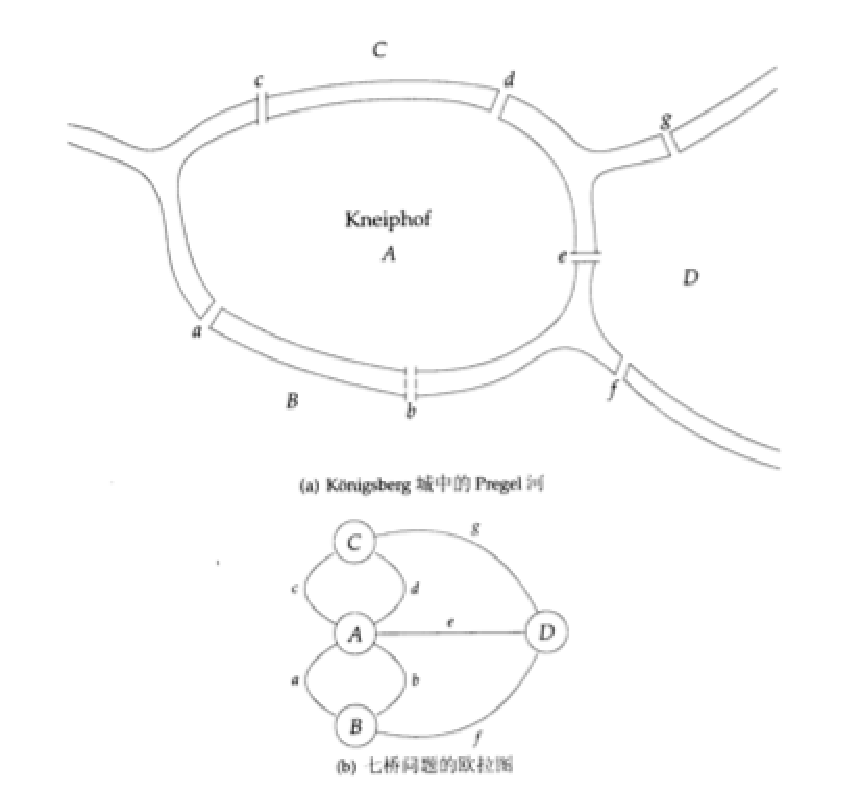
\includegraphics[width=5in]{fig/seven_bridges.pdf}
\end{figure}

四个区域用$A,B,C,D$标记,七座桥用$a,b,c,d,e,f,g$标记。七桥问题的提法是:从任何一个区域出发,跨过每座桥一次且一次,问最后能否回到出发的那个区域。

欧拉解决了这一问题,答案是不能。欧拉首先把这个问题描述为抽象的数学对象:图,用图的顶点表示区域,用图的边表示桥梁。图中顶点的度定义为与该顶点邻接的边数,欧拉证明了:如果从图中的一个顶点出发,经过图中所有边一次且仅一次,最后回到出发的顶点,那么当且仅当所有顶点的度都是偶数。后来为了纪念欧拉的发现,这样的回路称为欧拉回路。七桥问题之所以不存在欧拉回路,是因为所有顶点的度均为奇数。

\section{图的定义与术语}
图$G$由两个集合$V, E$组成,其中$V$是顶点的有限非空集合,$E$是顶点的二元组集合,顶点二元组称为边。$V(G)$和$E(G)$分别称为图$G$的顶点集和边集,以后也用$G=(V,E)$表示图。

\begin{figure}[htbp]
\centering
\begin{tikzpicture}[node distance=3cm,semithick,inner sep=1pt,bend angle=45,auto]
%\draw[help lines] (-3,-3) grid (3,0);
\node[state]   (v1)                     {1};
\node[state]   (v2) [below left  of=v1] {2};
\node[state]   (v3) [below right of=v1] {3};
\node[state]   (v4) [below left  of=v2] {4};
\node[state]   (v5) [below       of=v1] {5};
\node[state]   (v6) [below right of=v3] {6};
\node[state]   (v7) [below right of=v5] {7};
\node[state]   (v8) [right       of=v4] {8};
\node[state]   (v9) [below       of=v5] {9};

\path
(v1) edge node{} (v2)
     edge node{} (v3)
(v2) edge node{} (v4)
     edge node{} (v5)
     edge node{} (v8)
(v3) edge node{} (v5)
     edge node{} (v6)
(v4) edge node{} (v8)
     edge node{} (v9)
(v5) edge node{} (v7)
     edge node{} (v9)
(v6) edge node{} (v7)
(v7) edge node{} (v9)
(v8) edge node{} (v9);                     
\end{tikzpicture}
\end{figure}

注意:
\begin{itemize}
\item 
线性表的数据元素叫元素,树的数据元素叫结点,图的数据元素称为顶点(vertex)。 
\item 
线性表若无数据元素,称为空表。树中没有结点称为空树。但在图中,不允许没有顶点,即顶点集合$V$有限非空。
\end{itemize}

\noindent1、无向图
\begin{itemize}
\item 
若顶点$v_i$到$v_j$之间的边没有方向,则称该边为无向边(edge),用无序偶对$(v_i,v_j)$表示。 
\item
若图中任意两顶点之间的边都是无向边,则称该图为无向图(undirected graphs)。
\end{itemize}

\begin{figure}[htbp]
\centering
\tikzstyle{state}=[circle,draw=blue!50,fill=blue!20,thick,inner sep=0pt,minimum size=6mm]


\begin{tikzpicture}[node distance=2cm,semithick,bend angle=45,minimum size=0.1cm,draw,auto]
\node[state]   (a) at  (90:1) {$a$};
\node[state]   (b) at (180:1) {$b$};
\node[state]   (c) at (270:1) {$c$};
\node[state]   (d) at   (0:1) {$d$};
\path
(a) edge (b)
    edge (c)   
    edge (d)
(b) edge (c)
(c) edge (d);             
\end{tikzpicture}
\caption{无向图}
\end{figure}

\noindent2、有向图
\begin{itemize}
\item 
若顶点$v_i$到$v_j$之间的边有方向,则称这条边为有向边,也称为弧(arc),用有序偶对$<v_i,v_j>$表示,其中$v_i$称为弧尾(tail),$v_j$称为弧头(head)。 
\item
若图中任意两顶点之间的边都是有向边,则称该图为有向图(directed graphs)。
\end{itemize}

\begin{figure}
\centering
\tikzstyle{state}=[circle,draw=blue!50,fill=blue!20,thick,inner sep=0pt,minimum size=6mm]

\begin{tikzpicture}[->,>=stealth',shorten >=1pt,node distance=2cm,semithick,inner sep=1pt,bend angle=45,auto]
\node[state]   (A)                    {A};
\node[state]   (B) [below left  of=A] {B};
\node[state]   (C) [below right of=B] {C};
\node[state]   (D) [below right of=A] {D};
\path
(A) edge node{} (D)
(B) edge node{} (A)
    edge node{} (C)
(C) edge node{} (A);                     
\end{tikzpicture}
\caption{有向图}
\end{figure}

\noindent3、简单图:
若不存在顶点到自身的边,且同一条边不重复出现,则称这样的图为简单图。
\red{本章只讨论简单图。}

\begin{figure}[htbp]
\centering
\tikzstyle{state}=[circle,draw=blue!50,fill=blue!20,thick,inner sep=0pt,minimum size=6mm]
\begin{minipage}{0.45\textwidth}
\begin{tikzpicture}[scale=1.2,node distance=3cm,semithick,inner sep=1pt,bend angle=45,auto]
%\draw[help lines] (-3,-3) grid (3,0);
\node[state]   (a) at  (90:1) {$a$};
\node[state]   (b) at (180:1) {$b$};
\node[state]   (c) at (270:1) {$c$};
\node[state]   (d) at   (0:1) {$d$};
\path
(a) edge (b)
    edge (c)   
    edge[bend left=12] (d)
	 edge[bend right=12](d)
(b) edge (c)
(c) edge (d);             
\end{tikzpicture}
\end{minipage}
%%%%%%%%
\begin{minipage}{0.45\textwidth}
\begin{tikzpicture}[scale=1.2,->,>=stealth',node distance=3cm,semithick,inner sep=1pt,bend angle=45,auto]
%\draw[help lines] (-3,-3) grid (3,0);
\node[state]   (a) at  (90:1) {$a$};
\node[state]   (b) at (180:1) {$b$};
\node[state]   (c) at (270:1) {$c$};
\node[state]   (d) at   (0:1) {$d$};
\path
(a) edge (d)   
    edge[loop above] (A)
(b) edge (a)
    edge (c)
(c) edge (a);             
\end{tikzpicture}
\end{minipage}

\caption{非简单无向图}
\end{figure}

\noindent4、无向完全图:
在无向图中,若任意两顶点之间都存在边,则称该图为无向完全图。

\red{含有$n$个顶点的无向完全图有$\frac{n(n-1)}2$条边。}

\begin{figure}
\centering
\begin{tikzpicture}[scale=1.5,node distance=3cm,semithick,bend angle=45,minimum size=0.1cm,draw,auto]
%\draw[help lines] (-3,-3) grid (3,0);
\node[state]   (a) at  (90:1) {$a$};
\node[state]   (b) at (170:1) {$b$};
\node[state]   (c) at (260:1) {$c$};
\node[state]   (d) at (350:1) {$d$};
\path
(a) edge (b)
    edge (c)   
    edge (d)
(b) edge (c)
    edge (d)
(c) edge (d);             
\end{tikzpicture}
\caption{无向完全图}
\end{figure}


\noindent5、有向完全图:
在有向图中,若任意两顶点之间都存在方向相反的两条弧,则称该图为有向完全图。

\red{含有$n$个顶点的有向完全图有$n(n-1)$条弧。}

\begin{figure}
\centering
\begin{tikzpicture}[scale=1.5,node distance=3cm,semithick,bend angle=45,minimum size=0.1cm,draw,auto]
%\draw[help lines] (-3,-3) grid (3,0);
\node[state]   (a) at  (90:1) {$a$};
\node[state]   (b) at (170:1) {$b$};
\node[state]   (c) at (260:1) {$c$};
\node[state]   (d) at (350:1) {$d$};
\path
(a) edge[->,>=stealth',bend left=10]  (b)
    edge[<-,>=stealth',bend right=10] (b)
    edge[->,>=stealth',bend left=10]  (c)
    edge[<-,>=stealth',bend right=10] (c) 
    edge[->,>=stealth',bend left=10]  (d)
    edge[<-,>=stealth',bend right=10] (d)
(b) edge[->,>=stealth',bend left=10]  (c)
    edge[<-,>=stealth',bend right=10] (c)
    edge[->,>=stealth',bend left=10]  (d)
    edge[<-,>=stealth',bend right=10] (d)
(c) edge[->,>=stealth',bend left=10]  (d)
    edge[<-,>=stealth',bend right=10] (d);             
\end{tikzpicture}
\caption{有向完全图}
\end{figure}

对于具有$n$个顶点和$e$条边的图,无向图满足
$$
0\le e \le \frac{n(n-1)}2,
$$
有向图满足
$$
0\le e \le n(n-1).
$$

\noindent6、稠密图与稀疏图:
有很少条边或弧的图称为稀疏图,反之称为稠密图。

\red{这里稀疏与稠密是模糊概念,都是相对而言的。}

\noindent7、网络
\begin{itemize}
\item
有些图的边或弧具有与它相关的数字,这种与边或弧相关的数称为权(weight)。这些权可以表示从一个顶点到另一个顶点的距离或耗费。
\item
这种带权的图称为网(network)。
\end{itemize}

\begin{figure}
\centering
\tikzstyle{state}=[circle,draw=blue!50,fill=blue!20,thick,inner sep=0pt,minimum size=6mm]

\begin{tikzpicture}[scale=1.3,node distance=3cm,semithick,bend angle=45,minimum size=0.1cm,draw,auto]
%\draw[help lines] (-3,-3) grid (3,0);
\node[state]   (a) at (110:1.5) {北京};
\node[state]   (b) at (220:1.5) {香港};
\node[state]   (c) at (-45:1)   {台北};
\node[state]   (d) at  (45:1)   {上海};
\path
(a) edge node[near start,above]{\tiny 1463} (b)
    edge node[near start,below]{\tiny 2160}(c)   
    edge node[near start]{\tiny 1680}(d)
(b) edge node[near end,below]{\tiny  808}(c)
    edge node[midway,below]{\tiny 1200}(d)
(c) edge node[midway,right]{\tiny  700}(d);             
\end{tikzpicture}
\caption{网}
\end{figure}

\noindent8、子图:
假设有两个图$G=(V,E)$和$G^\prime=(V^\prime,E^\prime)$,如果$V^\prime\subset V$且$E^\prime\subset E$,则称$G^\prime$为$G$的子图(subgraph)。

\begin{figure}
\centering
\tikzstyle{state}=[circle,draw=blue!50,fill=blue!20,thick,inner sep=0pt,minimum size=6mm]

\begin{minipage}{\textwidth}
\begin{minipage}{0.35\textwidth}
\begin{tikzpicture}[scale=1.2,node distance=3cm,semithick,inner sep=1pt,bend angle=45,auto]
%\draw[help lines] (-3,-3) grid (3,0);
\node[state]   (a) at  (90:1) {$a$};
\node[state]   (b) at (180:1) {$b$};
\node[state]   (c) at (270:1) {$c$};
\node[state]   (d) at   (0:1) {$d$};
\path
(a) edge (b)
    edge (c)   
    edge (d)
(b) edge (c)
(c) edge (d);             
\end{tikzpicture}
\end{minipage}
%%%%%
\begin{minipage}{0.1\textwidth}
\begin{tikzpicture}[scale=1.2,node distance=3cm,semithick,inner sep=1pt,bend angle=45,auto]
%\draw[help lines] (-3,-3) grid (3,0);
\node[state]   (a) at  (90:1) {$a$};            
\end{tikzpicture}
\end{minipage}
%%%%%
\begin{minipage}{0.25\textwidth}
\begin{tikzpicture}[scale=1.2,node distance=3cm,semithick,inner sep=1pt,bend angle=45,auto]
%\draw[help lines] (-3,-3) grid (3,0);
\node[state]   (a) at  (90:1) {$a$};
\node[state]   (d) at   (0:1) {$d$};
\path
(a) edge (d);             
\end{tikzpicture}
\end{minipage}
%%%%%
\begin{minipage}{0.25\textwidth}
\begin{tikzpicture}[scale=1.2,node distance=3cm,semithick,inner sep=1pt,bend angle=45,auto]
%\draw[help lines] (-3,-3) grid (3,0);
\node[state]   (a) at  (90:1) {$a$};
\node[state]   (b) at (180:1) {$b$};
\node[state]   (c) at (270:1) {$c$};
\path
(a) edge (b)
    edge (c)   
(b) edge (c);
\end{tikzpicture}
\end{minipage}
\end{minipage} \vspace{0.05in}

%%%%%%%%
%%%%%%%%
\begin{minipage}{\textwidth}
\begin{minipage}{0.35\textwidth}
\begin{tikzpicture}[scale=1.2,->,>=stealth',node distance=3cm,semithick,inner sep=1pt,bend angle=45,auto]
%\draw[help lines] (-3,-3) grid (3,0);
\node[state]   (a) at  (90:1) {$a$};
\node[state]   (b) at (180:1) {$b$};
\node[state]   (c) at (270:1) {$c$};
\node[state]   (d) at   (0:1) {$d$};
\path
(a) edge (d)   
(b) edge (a)
    edge (c)
(c) edge (a);             
\end{tikzpicture}
\end{minipage}
%%%%
\begin{minipage}{0.1\textwidth}
\begin{tikzpicture}[scale=1.2,->,>=stealth',node distance=3cm,semithick,inner sep=1pt,bend angle=45,auto]
%\draw[help lines] (-3,-3) grid (3,0);
\node[state]   (a) at  (90:1) {$a$};           
\end{tikzpicture}
\end{minipage}
%%%%
\begin{minipage}{0.25\textwidth}
\begin{tikzpicture}[scale=1.2,->,>=stealth',node distance=3cm,semithick,inner sep=1pt,bend angle=45,auto]
%\draw[help lines] (-3,-3) grid (3,0);
\node[state]   (a) at  (90:1) {$a$};
\node[state]   (d) at   (0:1) {$d$};
\path
(a) edge (d);             
\end{tikzpicture}
\end{minipage}
\begin{minipage}{0.25\textwidth}
\begin{tikzpicture}[scale=1.2,->,>=stealth',node distance=3cm,semithick,inner sep=1pt,bend angle=45,auto]
%\draw[help lines] (-3,-3) grid (3,0);
\node[state]   (a) at  (90:1) {$a$};
\node[state]   (b) at (180:1) {$b$};
\node[state]   (c) at (270:1) {$c$};
\path
(b) edge (a)
    edge (c)
(c) edge (a);             
\end{tikzpicture}
\end{minipage}
\end{minipage}

\caption{子图}
\end{figure}

\section{顶点与边的关系}

\noindent 1、无向图顶点的邻接、度

对于无向图$G=(V,E)$,
\begin{itemize}
\item 
若边$(v,v^\prime)\in E$,则称$v,v^\prime$相邻,称边$(v,v^\prime)$邻接顶点$v$和$v^\prime$。 \item 
顶点$v$的度(degree)是和$v$邻接的边的数目,记为$D(v)$。 \item 重要关系:
$$
e=\frac12 \sum_{i=1}^n D(v_i).
$$
\end{itemize}
 

\noindent2、有向图顶点的邻接、入度、出度和度

对于有向图$G=(V,E)$,
\begin{itemize}
\item 
若弧$\langle v,v^\prime\rangle\in E$,则称$v$指向$v^\prime$,顶点$v^\prime$发自$v$,弧$\langle v,v^\prime\rangle$与$v,v^\prime$邻接。  
\item 
以$v$为头的弧的数目称为$v$的入度,记为$D_{in}(v)$;

以$v$为尾的弧的数目称为$v$的出度,记为$D_{out}(v)$;

顶点$v$的度为$D(v)=D_{in}(v)+D_{out}(v)$。 
\item 重要关系:
$$
e=\sum_{i=1}^n D_{in}(v_i)=\sum_{i=1}^n D_{out}(v_i).
$$
\end{itemize}
 
\noindent3、无向图的路径

对于无向图$G=(V,E)$,从顶点$v$到顶点$v^\prime$的路径(path)是一个顶点序列$(v=v_{i_0}, v_{i_1}, \cd, v_{i_m}=v^\prime)$,其中$(v_{i_{k-1}},v_{i_{k}})\in E, ~1\le k \le m$。

\tikzstyle{state}=[circle,draw=blue!50,fill=blue!20,thick,inner sep=0pt,minimum size=6mm]

\begin{figure}[htbp]
\centering
\begin{minipage}{0.45\textwidth}
\begin{tikzpicture}[scale=1.2,node distance=3cm,semithick,inner sep=1pt,bend angle=45,auto]
%\draw[help lines] (-3,-3) grid (3,0);
\node[state]   (a) at  (90:1) {$a$};
\node[state]   (b) at (180:1) {$b$};
\node[state]   (c) at (270:1) {$c$};
\node[state]   (d) at   (0:1) {$d$};
\path
(a) edge[very thick,red] (b)
    edge (c)   
    edge[very thick,red] (d)
(b) edge (c)
(c) edge (d);             
\end{tikzpicture}
\end{minipage}
%%%%%
\begin{minipage}{0.45\textwidth}
\begin{tikzpicture}[scale=1.2,node distance=3cm,semithick,inner sep=1pt,bend angle=45,auto]
%\draw[help lines] (-3,-3) grid (3,0);
\node[state]   (a) at  (90:1) {$a$};
\node[state]   (b) at (180:1) {$b$};
\node[state]   (c) at (270:1) {$c$};
\node[state]   (d) at   (0:1) {$d$};
\path
(a) edge (b)
    edge (c)   
    edge (d)
(b) edge[very thick,red] (c)
(c) edge[very thick,red] (d);             
\end{tikzpicture}
\end{minipage} \vspace{0.1in}



\begin{minipage}{0.45\textwidth}
\begin{tikzpicture}[scale=1.2,node distance=3cm,semithick,inner sep=1pt,bend angle=45,auto]
%\draw[help lines] (-3,-3) grid (3,0);
\node[state]   (a) at  (90:1) {$a$};
\node[state]   (b) at (180:1) {$b$};
\node[state]   (c) at (270:1) {$c$};
\node[state]   (d) at   (0:1) {$d$};
\path
(a) edge[very thick,red] (b)
    edge[very thick,red] (c)   
    edge (d)
(b) edge (c)
(c) edge[very thick,red] (d);             
\end{tikzpicture}
\end{minipage}
%%%%%
\begin{minipage}{0.45\textwidth}
\begin{tikzpicture}[scale=1.2,node distance=3cm,semithick,inner sep=1pt,bend angle=45,auto]
%\draw[help lines] (-3,-3) grid (3,0);
\node[state]   (a) at  (90:1) {$a$};
\node[state]   (b) at (180:1) {$b$};
\node[state]   (c) at (270:1) {$c$};
\node[state]   (d) at   (0:1) {$d$};
\path
(a) edge (b)
    edge[very thick,red] (c)   
    edge[very thick,red] (d)
(b) edge[very thick,red] (c)
(c) edge (d);             
\end{tikzpicture}
\end{minipage}

\caption{顶点$b$到$d$有四条路径}
\end{figure}

\noindent4、有向图的路径

对于有向图$G=(V,E)$,其路径也是有向的,顶点序列应满足$(v_{i_{k-1}},v_{i_{k}})\in E, ~1\le k \le m$。

\begin{figure}
\centering
\begin{minipage}{0.45\textwidth}
\begin{tikzpicture}[scale=1.2,->,>=stealth',node distance=3cm,semithick,inner sep=1pt,bend angle=45,auto]
%\draw[help lines] (-3,-3) grid (3,0);
\node[state]   (a) at  (90:1) {$a$};
\node[state]   (b) at (180:1) {$b$};
\node[state]   (c) at (270:1) {$c$};
\node[state]   (d) at   (0:1) {$d$};
\path
(a) edge[very thick,red]  (d)   
(b) edge[very thick,red]  (a)
    edge (c)
(c) edge (a);             
\end{tikzpicture}
\end{minipage}
%%%%%
\begin{minipage}{0.45\textwidth}
\begin{tikzpicture}[scale=1.2,->,>=stealth',node distance=3cm,semithick,inner sep=1pt,bend angle=45,auto]
%\draw[help lines] (-3,-3) grid (3,0);
\node[state]   (a) at  (90:1) {$a$};
\node[state]   (b) at (180:1) {$b$};
\node[state]   (c) at (270:1) {$c$};
\node[state]   (d) at   (0:1) {$d$};
\path
(a) edge[very thick,red]  (d)   
(b) edge (a)
    edge[very thick,red]  (c)
(c) edge[very thick,red]  (a);             
\end{tikzpicture}
\end{minipage}



\caption{顶点$b$到$d$有两条路径}
\end{figure}

\noindent5、路径长度

路径的长度是路径上的边或弧的数目。
 
\noindent6、回路或环

第一个顶点和最后一个顶点相同的路径称为回路或环(cycle)。

\noindent7、简单路径

序列中顶点不重复出现的路径称为简单路径。

\noindent8、简单回路或简单环
除第一个顶点和最后一个顶点外,其余顶点不重复的回路,称为简单回路或简单环。
 
\begin{figure}
\centering
\begin{minipage}{0.45\textwidth}
\begin{tikzpicture}[scale=1.5,node distance=3cm,semithick,inner sep=1pt,bend angle=45,auto]
%\draw[help lines] (-3,-3) grid (3,0);
\node[state]   (a) at  (90:1) {$a$};
\node[state]   (b) at (180:1) {$b$};
\node[state]   (c) at (270:1) {$c$};
\node[state]   (d) at   (0:1) {$d$};
\path
(a) edge[very thick,red](b) edge[->,above,blue,bend right=10]node{4}(b)
    edge(c)   
    edge[very thick,red](d) edge[<-,above,blue,bend left=10]node{3}(d)
(b) edge[very thick,red](c) edge[->,below,blue,bend right=10]node{1} (c)
(c) edge[very thick,red](d) edge[->,below,blue,bend right=10]node{2} (d);             
\end{tikzpicture}
\caption{简单回路}
\end{minipage}
%%%%%
\begin{minipage}{0.45\textwidth}
\begin{tikzpicture}[scale=1.5,node distance=3cm,semithick,inner sep=1pt,bend angle=45,auto]
%\draw[help lines] (-3,-3) grid (3,0);
\node[state]   (a) at  (90:1) {$a$};
\node[state]   (b) at (180:1) {$b$};
\node[state]   (c) at (270:1) {$c$};
\node[state]   (d) at   (0:1) {$d$};
\path
(a)edge (b)
   edge[very thick,red](c) edge[->,blue,bend right=10]node[left]{4}(c)   
   edge[very thick,red](d) edge[<-,blue,bend left=10]node{3}(d)
(b)edge[very thick,red](c) edge[->,blue,bend right=10]node[below]{1}(c) edge[<-,blue,bend left=10]node{5}(c)
(c)edge[very thick,red](d) edge[->,blue,bend right=10]node[below]{2}(d);             
\end{tikzpicture}
\caption{非简单回路}
\end{minipage}  


\end{figure}

\section{图的连通性}

\subsection{无向图的连通性}

\noindent1、连通图: 在无向图中,
\begin{itemize}
\item 
若顶点$v$到$v^\prime$有路径,则称$v$与$v^\prime$是连通的。  
\item
若对任意两个顶点$v_i,v_j\in E$,$v_i$和$v_j$都是连通的,则称$G$是连通图(connected graph)。
\end{itemize}
\begin{figure}
\centering
\begin{minipage}{0.45\textwidth}
\begin{tikzpicture}[scale=1.4,node distance=3cm,semithick,inner sep=1pt,bend angle=45,auto]
%\draw[help lines] (-3,-3) grid (3,0);
\node[state]   (a) at  (80:1) {$a$};
\node[state]   (b) at (170:1.5) {$b$};
\node[state]   (c) at (260:1) {$c$};
\node[state]   (d) at  (-10:1.5) {$d$};
\node[state]   (e) at (170:0.7) {$e$};
\node[state]   (f) at  (-15:0.5) {$f$};
\path
(a) edge (b)  
    edge (d)  
(b) edge (c) 
(c) edge (d)
(e) edge (f) ;             
\end{tikzpicture}
\caption{非连通图}
\end{minipage}
%%%%%
\begin{minipage}{0.45\textwidth}
\begin{tikzpicture}[scale=1.4,node distance=3cm,semithick,inner sep=1pt,bend angle=45,auto]
%\draw[help lines] (-3,-3) grid (3,0);
\node[state]   (a) at  (80:1) {$a$};
\node[state]   (b) at (170:1.5) {$b$};
\node[state]   (c) at (260:1) {$c$};
\node[state]   (d) at  (-10:1.5) {$d$};
\path
(a) edge (b)  
    edge (d)  
(b) edge (c) 
(c) edge (d) ;             
\end{tikzpicture}
\caption{连通图}
\end{minipage}  


\end{figure}

\noindent2、连通分量: 
无向图中的极大连通子图称为连通分量。

此概念强调 
\begin{itemize}
\item 
要是子图;  
\item
子图要是连通的; 
\item
连通子图含有极大顶点数; 
\item
具有极大顶点数的连通子图包含相关联于这些顶点的边。
\end{itemize}


\begin{figure}
\centering
\begin{minipage}{0.45\textwidth}
\begin{tikzpicture}[scale=1.2,node distance=3cm,semithick,inner sep=1pt,bend angle=45,auto]
%\draw[help lines] (-3,-3) grid (3,0);
\node[state]   (a) at  (80:1) {$a$};
\node[state]   (b) at (170:1.5) {$b$};
\node[state]   (c) at (260:1) {$c$};
\node[state]   (d) at  (-10:1.5) {$d$};
\node[state]   (e) at (170:0.7) {$e$};
\node[state]   (f) at  (-15:0.5) {$f$};
\path
(a) edge (b)  
    edge (d)  
(b) edge (c) 
(c) edge (d)
(e) edge (f) ;             
\end{tikzpicture}
\caption{非连通图}
\end{minipage}
%%%%%
\begin{minipage}{0.45\textwidth}
\begin{tikzpicture}[scale=1.2,node distance=3cm,semithick,inner sep=1pt,bend angle=45,auto]
%\draw[help lines] (-3,-3) grid (3,0);
\node[state]   (a) at  (80:1) {$a$};
\node[state]   (b) at (170:1.5) {$b$};
\node[state]   (c) at (260:1) {$c$};
\node[state]   (d) at  (-10:1.5) {$d$};
\path
(a) edge (b)  
    edge (d)  
(b) edge (c) 
(c) edge (d) ;             
\end{tikzpicture}
\caption{连通分量}
\end{minipage}  

\begin{minipage}{0.45\textwidth}
\begin{tikzpicture}[scale=1.2,node distance=3cm,semithick,inner sep=1pt,bend angle=45,auto]
%\draw[help lines] (-3,-3) grid (3,0);
\node[state]   (e) at (170:0.7) {$e$};
\node[state]   (f) at  (-15:0.5) {$f$};
\path
(e) edge (f) ;         
\end{tikzpicture}
\caption{连通分量}
\end{minipage}
%%%%%
\begin{minipage}{0.45\textwidth}
\begin{tikzpicture}[scale=1.2,node distance=3cm,semithick,inner sep=1pt,bend angle=45,auto]
%\draw[help lines] (-3,-3) grid (3,0);
\node[state]   (a) at  (80:1) {$a$};
\node[state]   (b) at (170:1.5) {$b$};
\node[state]   (c) at (260:1) {$c$};
\path
(a) edge (b)  
(b) edge (c);             
\end{tikzpicture}
\caption{不是连通分量}
\end{minipage} 


\end{figure}

\noindent3、连通图的生成树:
一个连通图的生成子树是一个极小的连通子图,它含有图中全部的$n$个顶点,但只有足以构成一棵树的$n-1$条边。
 

设无向图$G$有$n$个顶点, 
\begin{itemize}
\item
若边数小于$n-1$,则$G$是非连通图; 
\item
若边数大于$n-1$,则$G$必定构成一个环; 
\item
但边数等于$n-1$,并不一定是生成树。
\end{itemize}
 
\begin{figure}
\centering

\begin{tikzpicture}[scale=1.2,node distance=3cm,semithick,inner sep=1pt,bend angle=45,auto]
%\draw[help lines] (-3,-3) grid (3,0);
\node[state]   (a) at  (80:1.5) {$a$};
\node[state]   (b) at (170:2.5) {$b$};
\node[state]   (c) at (260:1.5) {$c$};
\node[state]   (d) at  (-10:2.5) {$d$};
\node[state]   (e) at (30:0.8) {$e$};
\node[state]   (f) at  (150:0.9) {$f$};
\node[state]   (g) at (220:0.8) {$g$};
\node[state]   (h) at  (320:0.8) {$h$};
\path
(a) edge (b)  
    edge (d)  
(b) edge (c) 
(c) edge (d)
(e) edge (f) 
    edge (d)
    edge (h)
(f) edge (g)
(g) edge (h);             
\end{tikzpicture}


\caption{普通无向图}
\end{figure}
 
\begin{figure}
\centering

\begin{tikzpicture}[scale=1.2,node distance=3cm,semithick,inner sep=1pt,bend angle=45,auto]
%\draw[help lines] (-3,-3) grid (3,0);
\node[state]   (a) at  (80:1.5) {$a$};
\node[state]   (b) at (170:2.5) {$b$};
\node[state]   (c) at (260:1.5) {$c$};
\node[state]   (d) at  (-10:2.5) {$d$};
\node[state]   (e) at (30:0.8) {$e$};
\node[state]   (f) at  (150:0.9) {$f$};
\node[state]   (g) at (220:0.8) {$g$};
\node[state]   (h) at  (320:0.8) {$h$};
\path
(a) edge (d)  
(b) edge (c) 
(c) edge (d)
(e) edge (f) 
    edge (d)
    edge (h)
(g) edge (h);             
\end{tikzpicture}


\caption{无向图的生成树}
\end{figure}
 
\begin{figure}
\centering

\begin{tikzpicture}[scale=1.2,node distance=3cm,semithick,inner sep=1pt,bend angle=45,auto]
%\draw[help lines] (-3,-3) grid (3,0);
\node[state]   (a) at  (80:1.5) {$a$};
\node[state]   (b) at (170:2.5) {$b$};
\node[state]   (c) at (260:1.5) {$c$};
\node[state]   (d) at  (-10:2.5) {$d$};
\node[state]   (e) at (30:0.8) {$e$};
\node[state]   (f) at  (150:0.9) {$f$};
\node[state]   (g) at (220:0.8) {$g$};
\node[state]   (h) at  (320:0.8) {$h$};
\path
(a) edge (b)  
(b) edge (c) 
(c) edge (d)
(e) edge (f) 
    edge (d)
(f) edge (g)
(g) edge (h);             
\end{tikzpicture}


\caption{无向图的生成树}
\end{figure}
 
\begin{figure}
\centering

\begin{tikzpicture}[scale=1.2,node distance=3cm,semithick,inner sep=1pt,bend angle=45,auto]
%\draw[help lines] (-3,-3) grid (3,0);
\node[state]   (a) at  (80:1.5) {$a$};
\node[state]   (b) at (170:2.5) {$b$};
\node[state]   (c) at (260:1.5) {$c$};
\node[state]   (d) at  (-10:2.5) {$d$};
\node[state]   (e) at (30:0.8) {$e$};
\node[state]   (f) at  (150:0.9) {$f$};
\node[state]   (g) at (220:0.8) {$g$};
\node[state]   (h) at  (320:0.8) {$h$};
\path
(a) edge (b)  
(b) edge (c) 
(c) edge (d)
(e) edge (f) 
    edge (h)
(f) edge (g)
(g) edge (h);             
\end{tikzpicture}


\caption{不是生成树}
\end{figure}

\subsection{有向图的连通性}

\noindent1、强连通图:
在有向图$G$中,若对$v_i,v_j\in V, v_i\ne v_j$,从$v_i$到$v_j$和从$v_j$到$v_i$存在路径,则称$G$是强连通图。有向图中的极大强连通子图称为有向图的强连通分量。
  
\begin{figure}
\centering
\begin{minipage}{0.45\textwidth}
\begin{tikzpicture}[scale=1.2,->,>=stealth',node distance=3cm,semithick,inner sep=1pt,bend angle=45,auto]
%\draw[help lines] (-3,-3) grid (3,0);
\node[state]   (a) at  (90:1) {$a$};
\node[state]   (b) at (180:1) {$b$};
\node[state]   (c) at (270:1) {$c$};
\node[state]   (d) at   (0:1) {$d$};
\path
(a) edge (d) 
    edge (b)   
(b) edge (c)
(c) edge (a);             
\end{tikzpicture}
\caption{非强连通图}
\end{minipage}
%%%%%
\begin{minipage}{0.45\textwidth}
\begin{tikzpicture}[scale=1.2,->,>=stealth',node distance=3cm,semithick,inner sep=1pt,bend angle=45,auto]
%\draw[help lines] (-3,-3) grid (3,0);
\node[state]   (a) at  (90:1) {$a$};
\node[state]   (b) at (180:1) {$b$};
\node[state]   (c) at (270:1) {$c$};
\path
(a) edge (b)   
(b) edge (c)
(c) edge (a);            
\end{tikzpicture}
\caption{强连通分量}
\end{minipage}



\end{figure}
 
 
\noindent2、有向树的生成森林
\begin{itemize}
\item 如果一个有向图恰有一个顶点的入度为0,其余顶点的入度均为1,则它是一棵有向树。 
\item
一个有向图的生成森林由若干棵有向树组成,含有图中全部顶点,但只有足以构成若干棵不相交的有向树的弧。
\end{itemize}
 
\begin{figure}
\centering

\begin{tikzpicture}[scale=1.2,->,>=stealth',node distance=3cm,semithick,inner sep=1pt,bend angle=45,auto]
%\draw[help lines] (-3,-3) grid (3,0);
\node[state]   (a) at (135:1.5) {$a$};
\node[state]   (b) at (180:2.3) {$b$};
\node[state]   (c) at (225:1.8) {$c$};
\node[state]   (d) at     (0:0) {$d$};
\node[state]   (e) at  (45:1.8) {$e$};
\node[state]   (f) at (350:2.5) {$f$};
\node[state]   (g) at (315:1.5) {$g$};
\path
(b) edge (a)  
    edge (c) 
(a) edge (d)
(c) edge (a)
(e) edge (d)
    edge (g) 
(f) edge (e)
    edge (g)
(g) edge (c)
    edge (d);
\end{tikzpicture}


\caption{普通有向树}
\end{figure}
 
\begin{figure}
\centering

\begin{tikzpicture}[scale=1.2,->,>=stealth',node distance=3cm,semithick,inner sep=1pt,bend angle=45,auto]
%\draw[help lines] (-3,-3) grid (3,0);
\node[state]   (a) at (135:1.5) {$a$};
\node[state]   (b) at (180:2.3) {$b$};
\node[state]   (c) at (225:1.8) {$c$};
\node[state]   (d) at     (0:0) {$d$};
\node[state]   (e) at  (45:1.8) {$e$};
\node[state]   (f) at (350:2.5) {$f$};
\node[state]   (g) at (315:1.5) {$g$};
\path
(b) edge (a)  
    edge (c) 
(a) edge (d)

(f) edge (e)
    edge (g);
\end{tikzpicture}


\caption{有向树的生成森林}
\end{figure}
 
%\subsection{小结}
% 
%\begin{itemize}
%\item 图按有无方向分为\red{无向图}和\red{有向图}。无向图由顶点和边构成,有向图由顶点和弧构成,弧有弧尾和弧头之分。\\[0.1in]
%\item 图按照边或弧的多少分为\red{稀疏图}和\red{稠密图}。如果任意两顶点之间都存在边叫\red{完全图},有向的叫\red{有向完全图}。若无重复的边和顶点到自身的边则叫\red{简单图}。\\[0.1in]
%\item 图中顶点之间有邻接、依附的概念。无向图顶点的边数叫做\blue{度},有向图顶点有\blue{入度}和\blue{出度}之分。\\[0.1in]
%\item 带权的图称为\red{网}。
%
%\end{itemize}•
%\end{frame}
%
%\begin{frame}\ft{\subsubsecname}
%\begin{itemize}
%\item 图中顶点间存在\blue{路径},两顶点存在路径则说明两顶点\blue{连通},如果路径最终回到起始点则称为\blue{环},当中不重复叫\blue{简单路径}。若任意两顶点都连通,则图就是\red{连通图},有向则称\red{强连通图}。图中有子图,若子图极大连通则为\blue{连通分量},有向的则称\blue{强连通分量}。\\[0.1in]
%\item 无向图中连通且含有$n$个顶点$n-1$条边的子图叫\blue{生成树}。有向图中一顶点入度为0其余顶点入度为1的叫\blue{有向树},一个有向图由若干棵有向树构成\blue{生成森林}。
%
%\end{itemize}•
%\end{frame}

\section{图的抽象数据类型}
\begin{lstlisting}[frame=tb]
ADT Graph
`数据对象:顶点的非空集合,由顶点二元组组成的边集`
`成员函数:`
   Graph Create()                      `return 空图`
   Graph InsertVertex(graph, v)        `在graph中插入v,然后return graph`
   Graph InsertEdge(graph, v1, v2)     `在graph中插入(v1,v2),然后return graph`
   Graph DeleteVertex(graph, v)        `在graph中删除v及其邻接边,然后return graph`
   Graph DeleteEdge(graph, v1, v2)     `在graph中删除(v1,v2),然后return graph`
   Boolean IsEmpty(graph)              `判断是否为空图`
   List Adjacent(graph, v)             `return与v相邻所有顶点的表`
end Graph
\end{lstlisting}
\end{document}  